\documentclass[spanish]{textolivre}

% metadata
\journalname{Texto Livre}
\thevolume{17}
%\thenumber{1} % old template
\theyear{2024}
\receiveddate{\DTMdisplaydate{2024}{3}{20}{-1}}
\accepteddate{\DTMdisplaydate{2024}{5}{4}{-1}}
\publisheddate{\DTMdisplaydate{2024}{7}{29}{-1}}
\corrauthor{Gema Alcaraz Mármol}
\articledoi{10.1590/1983-3652.2024.51693}
%\articleid{NNNN} % if the article ID is not the last 5 numbers of its DOI, provide it using \articleid{} commmand 
% list of available sesscions in the journal: articles, dossier, reports, essays, reviews, interviews, editorial
\articlesessionname{articles}
\runningauthor{Alcaraz Mármol}
%\editorname{Leonardo Araújo} % old template
\sectioneditorname{Hugo Heredia Ponce}
\layouteditorname{João Mesquita}

\title{Aprendizaje de lengua extranjera a través de herramientas digitales de corpus. Actitudes y autoeficacia en estudiantes universitarios del grado de Educación Primaria}
\othertitle{Aprendizagem de línguas estrangeiras através de ferramentas de corpus digital. Atitudes e autoeficácia em estudantes de licenciatura em Educação Primária}
\othertitle{Foreign language learning through digital corpus tools. Attitudes and self-efficacy in university students of Primary Education teacher training}

\author[1]{Gema Alcaraz Mármol~\orcid{0000-0001-7703-3829}\thanks{Email: \href{mailto:gema.alcaraz@uclm.es}{gema.alcaraz@uclm.es}}}
\affil[1]{Universidad de Castilla-La Mancha,  Departamento de Filología Moderna, Toledo, España.}

\addbibresource{article.bib}
\usepackage{array}

\begin{document}
\maketitle
\begin{polyabstract}
\begin{abstract}
El presente estudio tiene como objetivo explorar la
autoeficacia y actitudes sobre el uso de dos herramientas digitales de
corpus por parte de un grupo de estudiantes de inglés como lengua
extranjera que cursa el Grado en Educación Primaria en la Universidad de
Castilla-La Mancha. Los participantes realizaron una serie de
actividades en el contexto de la metodología basada en datos utilizando
como recurso dos herramientas de corpus: SKELL y BNC. Tras la
realización de las actividades y la manipulación de las herramientas de
corpus, los participantes respondieron un cuestionario donde debían
expresar su grado de acuerdo con cada una de las afirmaciones que
componían dicho cuestionario. El cuestionario hace referencia a aspectos
sobre la dificultad de uso, el nivel de utilidad, o la aplicación fuera
del aula de las herramientas digitales de corpus; también se pregunta a
los participantes por las actividades de aprendizaje basado en datos
para la adquisición de distintos aspectos de la lengua inglesa. Los
resultados apuntan a una actitud positiva y un nivel considerable de
autoeficacia hacia el corpus. Finalmente, se anima a adoptar este tipo
de metodología además de a una formación específica del profesorado para
su correcta y óptima aplicación.

\keywords{Autoeficacia \sep Aprendizaje basado en datos \sep Corpus \sep
	Actitudes \sep Lengua extranjera}
\end{abstract}

\begin{portuguese}
\begin{abstract}
O presente estudo tem como objetivo explorar a autoeficácia e
as atitudes face à utilização de duas ferramentas de \textit{corpus} digital por parte de um grupo de estudantes de inglês como língua estrangeira que
frequentam uma licenciatura em Educação Primária na Universidade de
Castilla-La Mancha. Os participantes realizaram uma série de atividades
no contexto da metodologia orientada para os dados, utilizando duas
ferramentas de corpus: SKELL e BNC. Após a realização das atividades e
a manipulação das ferramentas de \textit{corpus}, os participantes responderam a um questionário no qual tinham de expressar o seu grau de concordância com cada uma das afirmações que compunham o questionário. O questionário refere-se a aspectos de dificuldade de utilização, nível de utilidade ou aplicação fora da sala de aula das ferramentas de \textit{corpus} digital; os participantes são também questionados sobre atividades de aprendizagem baseadas em dados para a aquisição de diferentes aspectos da língua inglesa. Os resultados apontam para uma atitude positiva e um nível considerável de auto-eficácia em relação ao corpus. Por último,
incentiva-se a adoção deste tipo de metodologia, bem como a formação
específica de professores para a sua aplicação correta e optimizada.

\keywords{Auto-eficácia \sep Aprendizagem baseada em dados \sep \textit{Corpus} \sep Atitudes \sep Língua estrangeira}
\end{abstract}
\end{portuguese}

\begin{english}
\begin{abstract}
The present study aims to explore the self-efficacy and
attitudes towards the use of two digital corpus tools by a group of
students of English as a foreign language studying for a degree in
Primary Education at the University of Castilla-La Mancha. The
participants carried out a series of activities in the context of the
data-driven methodology using two corpus tools: SKELL and BNC. After
carrying out the activities and manipulating the corpus tools, the
participants answered a questionnaire in which they had to express their
degree of agreement with each of the statements that made up the
questionnaire. The questionnaire refers to aspects such as difficulty of
use, level of usefulness, or application outside the classroom of the
digital corpus tools; participants are also asked about data-driven
learning activities for the acquisition of different aspects of the
English language. The results point to a positive attitude and a
considerable level of self-efficacy towards the corpus. Finally, the
adoption of this type of methodology is encouraged as well as specific
teacher training for its correct and optimal application.


\keywords{Self-efficacy \sep Data-driven learning \sep Corpus \sep Attitudes \sep Foreign language}
\end{abstract}
\end{english}
\end{polyabstract}

\section{Introducción}\label{sec-Introducción}

La evolución de la inteligencia artificial (IA) ha marcado un hito
significativo en la actualidad sofocada por infodemia e infoxicación.
Esta transformación tecnológica, inicialmente concebida por John
McCarthy en 1956, ha avanzado significativamente, incorporando
aplicaciones de aprendizaje automático y procesamiento del lenguaje
natural (NLP) en herramientas educativas \cite{Sadiku2021}. No obstante, el gran salto se dio con la presentación de
ChatGPT en 2020, y con mejor respuesta a principios del 2023, siendo la
IA Generativa (IAGen) otra forma de entender a la IA; la IAGen crea
contenido original a partir de datos existentes mediante algoritmos y
redes neuronales avanzadas \cite{Feuerriegel2024}.

En el campo de la educación, los modelos de lenguaje grandes (LLM,
\emph{Large Language Model}), como ChatGPT \cite{OpenAI2023}, ha generado
diversos debates públicos y digitales como el de la opinión emitida por
el lingüista {\textcite{Chomsky2023}}, donde califica a ChatGPT como una forma de plagio de alta
tecnología, pudiendo socavar la educación al motivar a los estudiantes
en la búsqueda de atajos para la entrega de trabajos, como los ya
clásicos ensayos o resolución a preguntas cerradas, como en un
cuestionario de reforzamiento, por ejemplo. Ante este tipo de
reflexiones, han surgido otras como la de \textcite{Yell2023}, un
profesor retirado de la Universidad de Wisconsin, argumentan sobre que,
si se utiliza de forma adecuada, ChatGPT puede ser un recurso valioso
para fomentar el aprendizaje basado en la búsqueda e investigación,
permitiendo promover el pensamiento crítico. Aunque es indiscutible que
este tipo de tecnología es capaz de crear contenido nuevo en formato de
texto, imágenes o audio, permitiendo hasta asistir en tareas de
conocimiento y necesidades cotidianas \cite{Feuerriegel2024}.

La aplicación de ChatGPT en la educación se ve reflejada en el análisis
de \textcite{Dimitriadou2023}, quienes abordan la integración de la
IA en las aulas inteligentes y los desafíos éticos asociados, así como
en el estudio de \textcite{Tlili2023} abordando el uso de
\emph{chatbots}, que examinan la aplicación de ChatGPT en la elaboración
de ejercicios en forma de cuestionarios. Estos enfoques resaltan el
equilibrio necesario entre las capacidades de la IA y la intervención
humana para garantizar la relevancia, la exactitud y la equidad en la
educación.

Recientes investigaciones, como las de \textcite{Nasution2023} y \textcite{Ruiz2023},
han explorado el uso de ChatGPT 4.0 en la generación de ítems de examen,
destacando no solo su capacidad para crear preguntas de elección
múltiple relevantes y coherentes, sino también abordando desafíos como
irregularidades y redundancias en interacciones más prolongadas. Estos
estudios subrayan la importancia de la especificidad y sistematización
en los prompts para generar exámenes eficientes y precisos,
capitalizando las fortalezas de la IA para la educación \cite{Nasution2023, Ruiz2023}.

La investigación de \textcite{Nasution2023} se enfocó en la validez y
confiabilidad de las preguntas generadas por IA, un tema que ha
suscitado tanto interés como preocupación en la comunidad educativa. Con
una muestra de 272 estudiantes, Nasution emprendió la tarea de evaluar
una serie de preguntas creadas por ChatGPT, obteniendo resultados que
son tanto prometedores como reveladores. De las 21 preguntas generadas
por la IA, 20 resultaron ser válidas, lo que indica una alta tasa de
éxito. Este hallazgo es significativo, ya que subraya la capacidad de la
IA para producir contenido educativo que no solo es relevante, sino
también de calidad.

No obstante, también hay investigaciones en torno al uso de Machine
Learning (ML) como el de \textcite{Rauber2024} quienes desarrollaron un
modelo automatizado para medir el aprendizaje de conceptos y prácticas
de clasificación de imágenes mediante redes neuronales. Se basó en datos
de 240 estudiantes de secundaria y bachillerato, concluyendo que la
evaluación es confiable y válida. Además, destacaron la efectividad del
modelo resaltando la importancia de incluir ML en la educación escolar y
la capacidad del modelo para asistir en el proceso de evaluación,
facilitando la carga de trabajo de los docentes.

A medida que la tecnología de IA continúa evolucionando, con avances
significativos en las versiones más recientes de ChatGPT, se presenta
una oportunidad única para mejorar y sistematizar el proceso de creación
de exámenes. Las investigaciones de \textcite{Nasution2023,Ruiz2023} se
alinean con esta visión, proponiendo un enfoque metodológico que combina
la exploración y descripción detallada de las capacidades de ChatGPT 4.0
en la generación de ítems de examen, proporcionando así una perspectiva
integral de su aplicabilidad y eficacia en el ámbito educativo. No
obstante, todavía hacen falta estudios que comparen el comportamiento de
la IAGen y si los seres humanos somos capaces de detectar esas
diferencias, o bien, podrían ayudar a reducir la carga de los docentes e
instituciones al momento de crear exámenes de alto impacto; como los del
ingreso a la universidad.

Ante todos estos acontecimientos, y retomando estos modelos de lenguaje
que podrían ayudarnos a evaluar nuestra propia forma de comunicar, el
objetivo principal de esta investigación fue explorar y comparar la
eficacia de la IAGen, representada por ChatGPT 4.0, y los diseñadores
humanos en el desarrollo de ítems para el Examen de Ingreso a la
Educación Superior (ExIES), en el área de Lengua Escrita, a través del
método de juicio de expertos. Lo anterior, con el fin determinar la
calidad, relevancia y alineación de los ítems generados por ambas
fuentes (IA y humanos) con los estándares establecidos para la
evaluación educativa, centrándose en aspectos como claridad,
neutralidad, concisión, alineación curricular y adecuación de formato y
contenido.
\section{Marco Teórico}\label{sec-marcoteórico.tex}
\subsection{La lingüística de corpus en la enseñanza de lenguas extranjeras} \label{sub-sec-lingüísticadecorpus}

La lingüística de corpus está adoptando un papel cada vez más relevante
en la enseñanza y aprendizaje de lenguas extranjeras \cite{sinclair2004how,okeeffe2007corpus,romer2009corpus,szudarski2018corpus}. Así, ofrece herramientas y enfoques pedagógicos que
permiten al estudiantado manejar grandes cantidades de texto auténtico
en formato digital, obteniendo información útil sobre el significado de
palabras clave y determinadas estructuras gramaticales partiendo de su
contexto de uso \cite{hanks2013}. \textcite{mcenery2011what} diferencian entre
usos indirectos y directos del corpus en el marco de la enseñanza de
lenguas.

Tradicionalmente, la lingüística de corpus ha tenido un papel indirecto
en el aprendizaje, siendo fuente para el diseño de materiales didácticos
para lengua extranjera o para la confección de diccionarios de
aprendices donde, entre otros, se ofrece información concreta sobre la
frecuencia y contexto de uso de las palabras. Podemos encontrar otras
aplicaciones indirectas en el ámbito de las lenguas para fines
específicos, donde son comunes los glosarios derivados de corpus de
especialidad, por ejemplo. Además, y en la línea de las aplicaciones
indirectas, no podemos olvidar los corpus de aprendices, cuyo análisis
ofrece esclarecedores datos derivados de errores comunes, y que abren
una valiosa ventana a la que asomarse a la hora de investigar el proceso
de adquisición de lenguas extranjeras \cite{meunier2002pedagogical}.

Por otro lado, respecto a la aplicación directa de los corpus, también
denominado aprendizaje basado en datos, autores como \textcite{gabrielatos2005corpora}
y \textcite{bernardini2004corpora} destacan sus efectos positivos en la adquisición de
una lengua extranjera. En el aprendizaje basado en datos los aprendices
manejan herramientas de corpus, las cuales les permiten explorar el
comportamiento de la lengua meta en su contexto de uso real. Así,
observan la frecuencia de uso de las palabras y sus concordancias, entre
otros. Estos procedimientos desarrollan la capacidad del estudiantado
para identificar patrones lingüísticos, hacer generalizaciones
fundamentadas en la lengua que están aprendiendo y examinar en detalle
cierto léxico y estructuras morfosintácticas, contribuyendo así a su
competencia metalingüística. El proceso de enseñanza y aprendizaje
tiende así a convertirse en una experiencia más motivadora y auténtica,
puesto que el estudiante consolida conocimientos que ya posee, a la vez
que descubre e integra nuevos \cite{boulton2012what}.

\textcite{zapata-ros2018} destacan el papel que tienen las
herramientas digitales de corpus y el aprendizaje basado en datos en el
desarrollo de la capacidad reflexiva y de razonamiento del alumnado, que
se materializa en distintas destrezas cognitivas como analizar, hacer
inferencias, interpretar o verificar. Como bien apunta \textcite{boulton2009testing},
el aprendizaje basado en datos complementa el enfoque comunicativo ya
que fomenta, por un lado, el aprendizaje inductivo, y por otro la
autonomía del propio estudiantado. A este respecto, \textcite{flowerdew2015corpus}
menciona tres teorías de aprendizaje que fundamentan esta metodología:
la llamada Noticing Hypothesis o Hipótesis de la Captación, el
Constructivismo y la Teoría Sociocultural de \textcite{vygotsky1978mind}. Dichas teorías están presentes en el aprendizaje basado en datos y el uso de
corpus, puesto que mediante estos se construye conocimiento a partir de
la búsqueda y la observación, se aprende por notoriedad de patrones y se
refuerza la negociación de significado.

Al interactuar con los corpus, el estudiantado aplica destrezas de
pensamiento crítico que implican la observación, la conciencia
lingüística, la formulación, la comprobación de hipótesis, y la
sensibilidad a la variación lingüística. En una tarea típica de
aprendizaje basado en datos, el estudiantado examina un nodo (una
palabra o una cadena de palabras) y su contexto inmediato, tanto a la
izquierda como a la derecha, así como, si lo desea, el contexto más
amplio del párrafo. Cada nodo aparece en una denominada línea de
concordancia, y a partir de ahí se exploran las pruebas lingüísticas y
se construyen hipótesis sobre la naturaleza del uso de la lengua.

Se considera, por tanto, un enfoque constructivista, inductivo y
centrado en el alumnado, que fomenta la autonomía y el aprendizaje por
descubrimiento. En este contexto de enseñanza, el profesorado actúa como
asesor y guía, facilitando, más que transmitiendo, conocimientos
lingüísticos. Se presentan, por tanto, una combinación de innovaciones
tecnológicas, educativas y varios recursos en línea que promueven la
inclusión de diferentes perspectivas pedagógicas dentro y fuera del
aula. Así, contribuye a que el estudiantado universitario, actualmente
en su mayoría nativos digitales, aprecien los enfoques basados en corpus
y los adapten a su aprendizaje de lengua extranjera. Así, a través de
este tipo de aprendizaje el alumnado puede llegar a sus propias
conclusiones, con una retención más sólida y prolongada y un mayor
conocimiento de la lengua meta. En base a estas premisas, se podría
afirmar que el estudiantado es menos dependiente del profesorado, y
aprende directamente de la lengua en contexto real en lugar de hacerlo
de recursos tradicionales como los libros de texto, las gramáticas o los
diccionarios \cite{thomas2015deriving}.

Sin embargo, y a pesar de los numerosos estudios que defienden las
bondades del aprendizaje basado en datos, este enfoque no parece haber
recalado aún en las aulas de lengua extranjera. \textcite{callies2016towards} sugiere
que el profesorado requiere de una serie de competencias y conocimientos
para poder aplicar con éxito esta metodología: deben estar
familiarizados con la lingüística de corpus y las herramientas
digitales, además de tener una base de conocimientos lingüísticos en
general. Además, los profesores también deben poseer competencias
pedagógicas que les permitan aplicar los corpus en el proceso de
enseñanza, diseñando materiales adecuados y pedagógicamente sólidos,
combinándolos bien con otras técnicas de enseñanza e incorporándolas al
contexto educativo. Se puede afirmar que es necesario formar al
profesorado futuro y en activo para que desarrollen todas estas
competencias mencionadas arriba.

La reticencia de los docentes de lengua extranjera a aplicar el corpus
en sus clases ha sido bien documentada en los últimos años por autores
como \textcite{romer2009corpus} o \textcite{tribble2015teaching}. Estos autores realizaron encuestas a
un representativo número de docentes. Los resultados de sus
investigaciones apuntan, principalmente, a la falta de formación en este
tipo de metodología, aunque también se mencionan la falta de recursos y
herramientas de corpus accesibles, intuitivas y de bajo coste. La
mayoría de los docentes afirmaban desconocer las diferentes formas en
que los corpus se pueden explotar en el aula y las habilidades
necesarias para la aplicación de estos conocimientos. También es
interesante mencionar que el nivel educativo al que pertenezcan los
docentes influye en su visión sobre este enfoque. En un reciente estudio
llevado a cabo por \textcite{crosthwaite2021voices}, docentes de inglés de
primaria y secundaria en Indonesia participaron en un taller formativo
sobre corpus y aprendizaje basado en datos. Tras preguntar a los
participantes por sus impresiones, los investigadores detectaron una
clara diferencia entre las opiniones de docentes de distintas etapas
educativas. Mientras que los profesores de secundaria veían cierto
potencial en el enfoque, aunque con ciertas reticencias, los de primaria
se mostraban mucho menos atraídos por este tipo de enseñanza en general.

No obstante, la investigación sobre el corpus y el aprendizaje basado en
datos ha dado resultados satisfactorios en cuanto a su acogida por parte
de alumnado. \textcite{geluso2014discovering} estudiaron las opiniones de un
grupo de estudiantes de inglés como lengua extranjera que utilizaron
herramientas de corpus para trabajar sus destrezas orales. Tras realizar
varias actividades, respondieron a un cuestionario tipo Likert donde se
les preguntaba sobre su experiencia. La mayoría de ellos consideraban
dichas herramientas como muy útiles pese a la novedad y el tiempo
empleado en saber utilizarlas adecuadamente. En la misma línea, los
estudios de \textcite{asik2016lexical} y \textcite{lin2016effects} destacan la buena
actitud demostrada por el estudiantado tras haber experimentado la
metodología de aprendizaje basado en datos. En el primer estudio, además
de un cuestionario, los participantes se sometieron a una entrevista en
grupo, donde mostraron una actitud muy positiva hacia esta metodología,
especialmente a la hora de trabajar con sinónimos y colocaciones.

En \textcite{lin2016effects}, tanto estudiantes de grado como de posgrado afirmaron
sentirse más autónomos y protagonistas de su proceso de aprendizaje. En
esta investigación se aplicaron tres acciones formativas: en la primera,
únicamente se trabajó con herramientas de corpus, en la segunda y
tercera acción formativa se combinó el aprendizaje basado en datos con
una metodología tradicional en distintas proporciones para cada grupo.
Si bien la actitud positiva se detectó en las tres acciones formativas,
fue en el primer grupo donde se obtuvieron las actitudes más favorables.
Las herramientas de corpus se utilizaron como base para el aprendizaje
de lengua extranjera a través de aplicaciones móviles. En este sentido,
\textcite{perezparedes2019mobile} quisieron saber si el uso de
herramientas de corpus en este tipo de dispositivo tenían la misma
acogida que en contextos de aula. Los resultados mostraron que, si bien
los usuarios sugirieron mejoras referentes al diseño de algunas
actividades, quedaron muy satisfechos con este tipo de aprendizaje.

\subsection{Autoeficacia en el aprendizaje de lenguas extranjeras}\label{sub-sec-autoeficaciaenelaprendizajedelenguas extranjeras}

Uno de los conceptos relacionados con las creencias y actitudes respecto
al aprendizaje es la autoeficacia. La literatura de los últimos veinte
años ha resaltado la importancia de las diferencias individuales a la
hora de abordar el proceso de enseñanza y aprendizaje de una lengua
extranjera \cite{chamorro2021actitudes,dornyei2019towards,munoz2019actitudes,you2016}. Autores como \textcite{dornyei2019towards} sugieren que, además de las aptitudes
y capacidades cognitivas de los aprendices, factores como la motivación,
las creencias y otras individualidades tienen un papel fundamental para
que un aprendiz tenga éxito en su adquisición de una lengua extranjera.
No obstante, el concepto de autoeficacia ha sido de estudio
relativamente reciente, comparado con otros factores individuales.

La autoeficacia comenzó a despertar interés a finales de los años 80 con
estudios en el marco de la teoría sociocognitiva de la mano de
investigaciones como las de \textcite{bandura1986social}. Sus investigaciones se
centran en explorar cómo lo que los individuos piensan de sí mismos y
del entorno influye en su manera de comportarse y de afrontar la
realización de determinadas tareas \textcite{bandura1986social}. En una reciente
definición \textcite{lin2014learning} concibe la autoeficacia como la confianza que una
persona tiene sobre ella misma respecto a su propia capacidad para
realizar una tarea, determinando así la cantidad de esfuerzo y tiempo
que está dispuesta a dedicar a dicha tarea. Investigaciones como la de
\textcite{linnenbrink2003role} han observado cómo la autoeficacia ayuda
de manera significativa en los procesos de aprendizaje a nivel tanto
cognitivo como motivacional.

La autoeficacia se ha relacionado con el uso de estrategias de
aprendizaje. \textcite{li2010empirical}, \textcite{anam2016language} o \textcite{saito2020strategy}
observaron que los aprendices con mayores niveles de autoeficacia hacían
uso de más y mejores estrategias de aprendizaje. De la misma manera,
\textcite{haro2021soler2021} explora los beneficios de la autoeficacia para alumnado de
traducción. Más concretamente en el campo de las lenguas extranjeras, la
relación entre la autoeficacia y el uso de estrategias es una de las
líneas más exploradas. Entre los estudios más recientes encontramos a
\textcite{tengwangwu2021metacognitive} o \textcite{bai2023role}. El primero de los estudios
es especialmente significativo dado el número de estudiantes que
formaron parte del mismo. Más de 500 estudiantes de inglés de origen
chino realizaron una encuesta donde se les preguntaba por diferentes
estrategias y aspectos motivacionales. Los resultados revelaron que la
autoeficacia predecía especialmente el uso de estrategias metacognitivas
y aumentaba la motivación por aprender en una época particularmente
complicada para la docencia como fue la pandemia por covid-19. En un
estudio incluso más reciente, \textcite{bai2023role} comprobaron que no solo
las estrategias como la planificación o la automonitorización se veían
favorecidas por la autoeficacia, sino también la motivación intrínseca
de los participantes a la hora de realizar distintas tareas en lengua
inglesa.

También encontramos investigaciones que muestran cómo la autoeficacia es
un buen predictor para determinar el éxito del estudiantado a la hora de
realizar ciertas actividades. Por ejemplo, \textcite{waddington2019developing} exploró qué
tareas comunicativas estaban más afectadas por un bajo nivel de
autoeficacia. Llegó a la conclusión de que tanto las destrezas
receptivas como las productivas se vieron mermadas por esa falta de
autoeficacia. Por su parte, \textcite{sardegna2018self} observaron que
un alto nivel de autoeficacia mejoraba los resultados de aprendizaje en
términos de pronunciación. Es la destreza de producción escrita la que
ha sido más explorada en este contexto. Como ejemplos podemos mencionar
a \textcite{woodrow2011college}, \textcite{villalon2013high} o \textcite{teng2021individual}. El
primero observó que la mayoría de los participantes presentaba cierto
grado de ansiedad a la hora de enfrentarse a una tarea escrita en
inglés. Los resultados del estudio apuntaban a que esa relación estaba
condicionada por la autoeficacia. Es decir, aquellos estudiantes con más
nivel de autoeficacia manejaban mejor sus niveles de ansiedad a la hora
de realizar la producción escrita. Por su parte, \textcite{villalon2013high} introdujeron la variable del género, queriendo averiguar
si había diferencias significativas entre estudiantes del género
femenino y masculino a la hora de cómo lidiaban con sus tareas de
producción escrita según una mayor o menor autoeficacia. Los
investigadores no encontraron diferencias significativas entre ambos
géneros, si bien confirmaban estudios anteriores respecto al papel de la
autoeficacia en la producción escrita en lengua extranjera. En la línea
de los dos anteriores, el trabajo de \textcite{teng2021individual} muestra que el nivel de
autoeficacia está íntimamente ligado tanto a estrategias cognitivas como
metacognitivas utilizadas en las tareas escritas.

Como se ha discutido arriba, los estudios que se refieren a la
autoeficacia en el contexto de enseñanza y aprendizaje de una lengua
extranjera se centran en la relación de esta con ciertas destrezas
comunicativas y con otras diferencias individuales como son la ansiedad
o la motivación. Sin embargo, y a pesar del interés que despierta dicha
autoeficacia actualmente en el aprendizaje de lenguas extranjeras,
faltan estudios que exploren su papel en el contexto de distintas
metodologías de enseñanza como puede ser las que adoptan herramientas
digitales de corpus.
\section{Objetivo de la Investigación}\label{sec-objetivodelainvestigación}

La presente investigación tiene como objetivo conocer el nivel de
autoeficacia y actitudes de un grupo de estudiantes del grado de
Educación Primaria, respecto a la metodología basada en datos y el uso
de las herramientas digitales de corpus.

La novedad de nuestro estudio radica, por tanto, en dos aspectos. Por un
lado, explora la autoeficacia en un contexto de aprendizaje basado en
datos. Esta metodología de implantación aún incipiente en el contexto de
enseñanza de lengua extranjera hace uso de herramientas de corpus
digitales como recurso de aula manipulable para el alumnado.

Por otro lado, el perfil de los participantes es concreto. La muestra
está formada por estudiantes universitarios, futuros docentes de lengua
extranjera en la etapa de educación primaria. Si bien es cierto que los
estudios tanto de autoeficacia como de aprendizaje basado en datos se
dan en contextos de enseñanza superior, el hecho de que sean futuros
docentes de lengua extranjera puede aportar una visión particular, la
cual no pueden proporcionar otras investigaciones cuya muestra es
estudiantado de otros grados universitarios. Es decir, hablamos de
docentes de lengua extranjera en formación, que podrán aplicar la
metodología basada en datos y las herramientas de corpus en un futuro
cercano. La opinión y actitudes que tengan sobre dicha metodología y
recursos puede determinar el papel de los mismos en las aulas de lengua
extranjera.
\section{Metodologia}\label{sec-metodologia}

Não foi necessária uma análise ética prévia por parte dos conselhos de
projetos adequados para a investigação, uma vez que os participantes não
foram identificados. Por não haver conflito de interesses, a Texto Livre
não terá quaisquer consequências, inclusive assistência integral e
eventual, ressarcimento de qualquer dano resultante a qualquer dos
participantes da pesquisa, conforme a Resolução nº 510, de 7 de abril de
2016, do Conselho Nacional de Saúde do Brasil.

A metodologia é a explicação minuciosa, detalhada, rigorosa e exata de
toda a ação desenvolvida no método de trabalho da pesquisa \cite{lakatos2003}. A pesquisa é um estudo de caso, que teve o aluno como
objeto de estudo. \textcite[p. 32]{yin2005} argumenta que o estudo de caso visa a \enquote{conhecer em profundidade o como e o porquê de uma determinada
	situação que se supõe ser única em muitos aspectos, procurando descobrir
	o que há nela de mais essencial e característico}. O estudo de caso é
caracterizado pelo estudo profundo e exaustivo de um ou poucos objetos,
de maneira a permitir o seu conhecimento amplo e detalhado. O caso
experimental caracteriza-se por determinar um objeto de estudo,
selecionar as variáveis que seriam capazes de influenciá-lo, definir as
formas de controle e de observação dos efeitos que a variável produz no
objeto \cite{gil2002}. A coleta dos dados foi realizada em uma escola
secundária do sul de Moçambique. Fizeram parte da amostra 50 alunos do
ensino secundário, selecionados de forma aleatória, dos quais 25
participaram do estudo das PO e aplicação do Q3DM. Os restantes 25
estiveram envolvidos no estudo das SCs e aplicação do GeoGebra. Em ambos
os estudos, todos os alunos experimentaram as aplicações (Q3DM ou
GeoGebra). A pesquisa apresenta um estudo de caso interpretativo, o qual
desenvolve categorias conceituais indutivamente para examinar os
pressupostos iniciais, as intenções e significados das ações e
expressões dos alunos \cite{amado2017}. A compreensão interpretativa é
sustentada a partir do relato pormenorizado da interação dos sujeitos em
seu meio natural \cite{coulon1995}. A visão interpretativa descreveu as
ações dos alunos em ambiente de sala de aula e os significados das ações
no processo de toda a pesquisa \cite{coutinho2011}.

Foi possível, pois, observar e interpretar tudo o que ocorreu, tornando
viável a análise das relações causa-efeito. Foi possível , também,
qualificar as ações dos alunos em todo o processo de aprendizagem, por
meio das interpretações dos significados de seus comportamentos durante
a mediação da aula e as respostas do questionário de satisfação. Além
disso, os dados foram coletados por meio das técnicas de observação do
participante, com tomada de notas e de registro fotográfico, assim como
dos instrumentos de coleta de dados aplicados, como os questionários de
satisfação.

\subsection{Realização das aulas}\label{sub-sec-Realização das aulas}

As aulas consistiram na apresentação de dois temas, PO e SCs, de forma
separada. Para os alunos da 9ª classe, o tema de pesquisa foi PO, e foi
utilizado o Q3DM. A professora primeiramente apresentou o tema,
explicando o que eram POs, dizendo que eram figuras geométricas sobre um
plano que poderiam ser comparadas à sombra do mesmo objeto no horário em
que o sol estaria no ponto mais alto no dia. Depois, demonstrou as
vistas ortogonais do sólido. (Ver \Cref{fig-03}).

\begin{figure}[htpb]
\centering
\begin{minipage}{.5\textwidth}
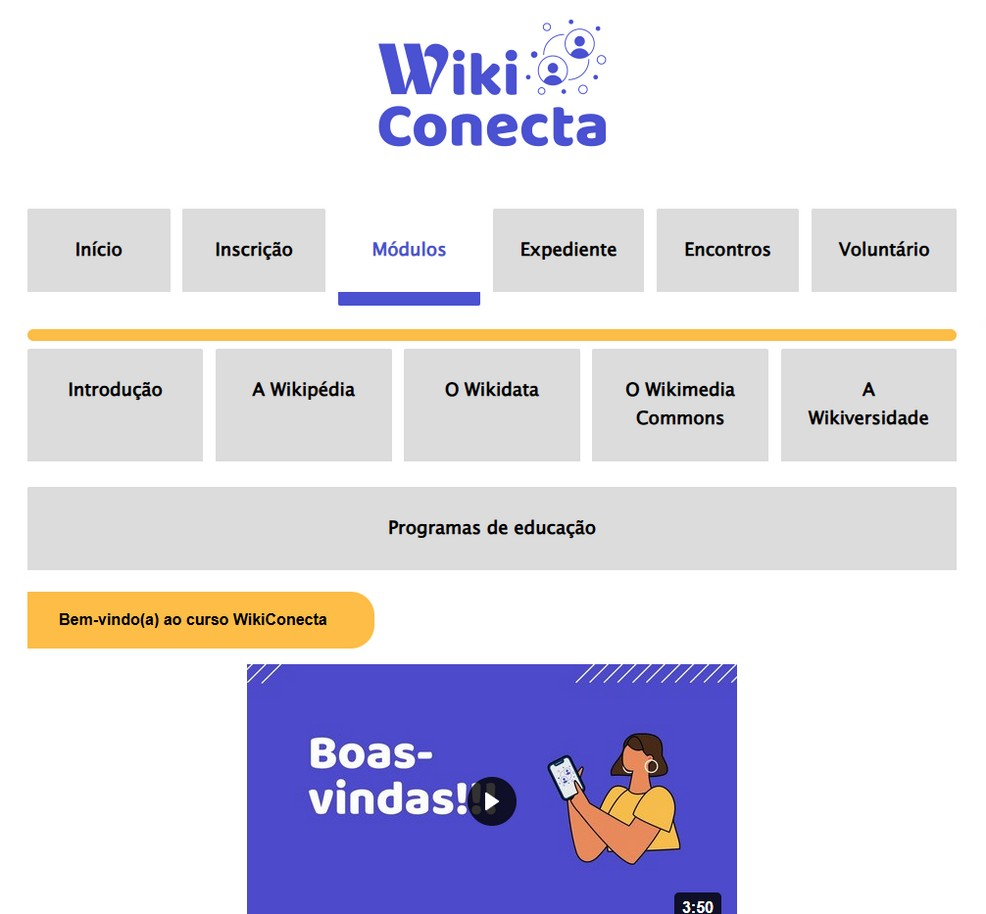
\includegraphics[width=\textwidth]{figures/figure03.jpg}
\caption{Vistas ortogonais e ortográficas: vista frontal; vista superior; e vista lateral esquerda.}
\label{fig-03}
\source{\url{http://turmag1215vialonga.blogspot.com/2014/10/projecoes-ortogonais.html}.}
\end{minipage}
\end{figure}

Posteriormente a professora apresentou a aplicabilidade das POs, dizendo
que eram destinadas à planificação de vários objetos. Com o auxílio das
simulações computacionais, construiu os sólidos geométricos e demonstrou
suas vistas ortogonais, apresentando os procedimentos para a manipulação
do Q3DM. (Ver \Cref{fig-04})

\begin{figure}[htpb]
\centering
\begin{minipage}{.5\textwidth}
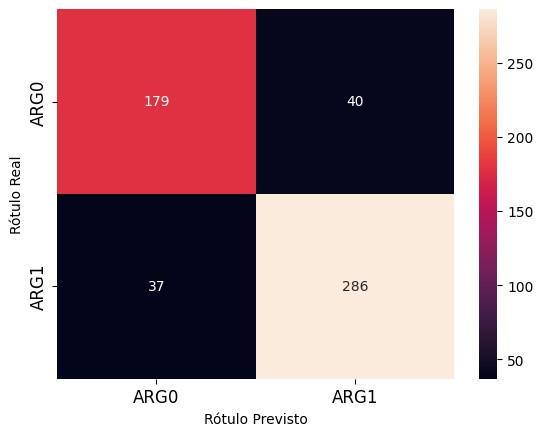
\includegraphics[width=\textwidth]{figures/figure04.jpg}
\caption{Manipulação no Q3DM.}
\label{fig-04}
\source{Elaboração própria.}	
\end{minipage}
\end{figure}


A manipulação no Q3DM é feita por meio de cubos chamados Qubes, que
facilitam a criação e a montagem de objetos em três dimensões,
utilizando elementos digitais que podem ser inseridos, removidos,
deslocados, ampliados, inclinados, moldados geometricamente, girados e
coloridos.

Para os alunos da 12ª classe, o tema de pesquisa foi SCs e foi utilizado
o GeoGebra. A professora iniciou com a apresentação do tema SCs de
cilindro, explicando que a seção cilíndrica é uma figura resultante de
um plano secante no cilindro. A professora acrescentou que existem duas
situações distintas: quando o plano secante é paralelo ao eixo central
do cilindro; e quando o plano secante não é paralelo ao eixo central do
cilindro (ver as figuras \Cref{fig-05} e \Cref{fig-06}).

\begin{figure}[htpb]
\centering
\begin{minipage}{.25\textwidth}
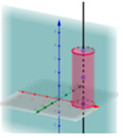
\includegraphics[width=\textwidth]{figures/figure05.jpg}
\caption{Secção paralela ao eixo central do cilindro.}
\label{fig-05}
\source{Elaboração própria.}
\end{minipage}
\end{figure}

\begin{figure}[htpb]
\centering
\begin{minipage}{.5\textwidth}
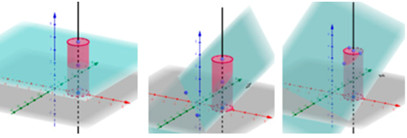
\includegraphics[width=\textwidth]{figures/figure06.jpg}
\caption{Secção não paralela ao eixo central do cilindro.}
\label{fig-06}
\source{Elaboração própria.}
\end{minipage}
\end{figure}

A professora, primeiramente, apresentou os diferentes posicionamentos
dos planos em relação ao eixo central do cilindro. Em seguida, com o
auxílio da tecnologia, apresentou à turma o software de geometria
dinâmica GeoGebra, indicando as funcionalidades de suas ferramentas e
como construir do ponto até o plano secante, com a ajuda dos
procedimentos para a sua manipulação no GeoGebra. Os alunos simularam as
SCs com o plano de nível; eles apresentaram-se atentos e motivados em
aprender a resolver o exercício no GeoGebra, particularmente para os
rapazes, os quais procuravam descobrir como construir diferentes sólidos
geométricos e como simular as VOs (vistas ortogonais).

\subsection{Realização do questionário}\label{sub-sec-Realização do questionário}

O questionário de satisfação aplicado teve como objetivo compreender se
o Q3DM e o GeoGebra facilitaram a aprendizagem das POs e SCs, e se o
\textit{smartphone} foi fácil de manipular. Ambos os questionários foram
preenchidos em 10 minutos. As questões visavam a coletar, nos dois
estudos, várias opiniões, incluindo: (1) se os aplicativos tecnológicos
facilitaram as representações 3D; (2) qual é a opinião deles sobre os
benefícios de usar os aplicativos ou se seria melhor resolver de forma
tradicional; (3) se os aplicativos são fáceis e intuitivos de usar; (4)
quais foram os aspectos positivos e negativos da aula; e, (5) como eles
classificariam a aprendizagem com o auxílio dos aplicativos.

\section{Resultados y discusión}\label{sec-resultadosydiscusión}

La mayoría de los participantes afirmaron que trabajar con herramientas
digitales de corpus y realizar actividades de aprendizaje basado en
datos aumentaba sus expectativas respecto a su aprendizaje del inglés.
Así, un 63,6~\% se mostró, de alguna manera, de acuerdo al afirmar que
sentían que las herramientas de corpus les hacían avanzar en su proceso
de aprendizaje, mientras que, de manera similar, un porcentaje del 75,7~\% comentó lo mismo respecto a las actividades de aprendizaje basado en
datos. En general, el 93,9~\% recomendaría el uso de herramientas de
corpus para aprender inglés, incluso más de un 27,3~\% afirmó que estaba
no sólo de acuerdo sino muy de acuerdo con esta afirmación. Estas
afirmaciones son positivas para el aprendizaje desde el punto de vista
motivacional. De hecho \textcite{raoofi2012self} argumentan que el
creer que se es capaz de hacer una tarea aumenta significativamente las
posibilidades de éxito en dicha tarea. De manera similar, tras un
meta-análisis de los estudios más relevantes sobre la relación entre
autoeficacia y nivel de lengua extranjera, \textcite{wang2020} concluyeron
que a mayor nivel de autoeficacia, mayor competencia lingüística.

Estas respuestas están en consonancia con el estudio de \textcite{lin2016effects},
donde tras la aplicación de la nueva metodología los participantes
afirmaban haber mejorado en cuanto a sus creencias de lo que podían ser
capaces de aprender y hacer en la lengua extranjera. Así, no se debe
pasar por alto el papel de la autoeficacia y el autoconcepto del
estudiante de cara al éxito en su proceso de aprendizaje.
Investigaciones como la de \textcite{sun2020college} y \textcite{genc2016exploring}
muestran cómo este tipo de factores afectivos pueden llegar a ser
importantes predictores del desarrollo de la adquisición de una segunda
lengua. Por tanto, el hecho de que la metodología basada en datos y las
herramientas de corpus parezcan contribuir a aumentar el nivel de
autoeficacia del estudiantado nos muestra el potencial de estas como
elemento de refuerzo en el aprendizaje de la lengua extranjera.

Al preguntar por su capacidad de aprendizaje de inglés a través de esta
nueva metodología y recursos, una amplia mayoría afirmó sentirse capaz
de hacerlo y de tener éxito (94~\%). De manera más específica, el
cuestionario planteó afirmaciones respecto a la adquisición de
vocabulario, gramática y expresiones idiomáticas en la lengua inglesa
(los tres contenidos que se habían trabajado a través de corpus en el
estudio). La mayoría se veía capaz de mejorar los tres aspectos gracias
a dichos recursos digitales. Los participantes se vieron especialmente
capaces de mejorar el aprendizaje de vocabulario (100~\%), seguido de
las expresiones idiomáticas (94~\%) y por último la gramática (81,8~\%).
Estudios anteriores están en la línea de los resultados obtenidos aquí.
Por ejemplo, \textcite{saeedakhtar2020effect} constataron un cambio de
actitud hacia el aprendizaje de colocaciones entre estudiantes
universitarios de inglés como lengua extranjera. Tras una intervención
didáctica basada en el uso de recursos digitales de corpus, los
participantes afirmaron tener más ánimo de seguir estudiando
colocaciones a través de dicha metodología. Otras dos investigaciones
llevadas a cabo por \textcite{yao2019vocabulary} y \textcite{sinha2021efl} se centraron en el uso de
herramientas de corpus para el aprendizaje de léxico en segunda lengua.
También en estos casos los participantes mostraron una actitud muy
positiva hacia este tipo de recursos. Por último, \textcite{charles2014getting} o
\textcite{guilquin2021using} realizaron encuestas de satisfacción y actitud tras
aplicar herramientas de corpus para el aprendizaje de ciertas
construcciones gramaticales. Descubrieron que no solo la actitud era
positiva sino que realmente esta metodología basada en datos y el corpus
como recurso didáctico suponían una diferencia significativa en cuanto
al aprendizaje de dichas estructuras gramaticales.

Los participantes valoraron ocho afirmaciones sobre la dificultad,
utilidad, uso fuera y dentro de clase, entre otras, referidas a las
herramientas digitales de corpus y la metodología de aprendizaje basado
en datos. En cuanto a la dificultad del uso de las herramientas de
corpus, más de la mitad de los participantes se mostraron en desacuerdo
(54,4~\%) con la afirmación de que las herramientas eran difíciles de
utilizar. Nuestros resultados coinciden con estudios anteriores como el
de \textcite{daskalovska2015corpus}, que observó que los participantes de su estudio
habían manejado las herramientas digitales de corpus con una destreza
bastante alta, a pesar de que habían recibido una formación muy básica
sobre ellas, como ocurre en este estudio. Incluso con ese grado mínimo
de familiarización, la autora pudo comprobar que el estudiantado había
sacado partido a las herramientas. Una de las razones podría ser, entre
otras, la edad de los participantes. Tanto los del estudio de
Daskalovska como los nuestros pertenecen a la generación de nativos
digitales, los cuales de manera intuitiva se hacen en poco tiempo con
todo tipo de recursos digitales.

Preguntados por si consideraban dichas herramientas más útiles que otros
recursos que ya utilizaban, el 87,9~\% estuvo de acuerdo en que sí.
Además, manifestaron su deseo de seguir aprendiendo más sobre estas
herramientas digitales de corpus el 90,9~\%, de los cuales un 27,3~\%
respondió estar ``muy de acuerdo'' con esta afirmación. En cuanto a su
opinión sobre las actividades de aprendizaje basado en datos, el 69,7~\%
afirmó no encontrarlas aburridas, además de preferirlas a actividades
más tradicionales que se solían hacer en clase con una amplia mayoría
del 87,8~\%.

Por otro lado, deseaban seguir utilizando dichas herramientas tanto
dentro como fuera de clase en la mayor parte de los casos. Preguntados
sobre hasta qué punto estaban de acuerdo en utilizar de forma regular
las herramientas de corpus en el aula, el 63,6~\% respondió estar de
acuerdo e incluso muy de acuerdo. En el caso de si les gustaría
incorporar dichas herramientas a su aprendizaje fuera del aula, la
respuesta también fue muy positiva con el 57,5~\% de participantes
respondiendo que estaban de acuerdo o muy de acuerdo con ello. Los datos
aquí recabados son especialmente relevantes en el sentido de que estos
mismos participantes van a ser docentes de inglés en un futuro próximo.
Por tanto, el haber tenido una buena experiencia con las herramientas de
corpus los puede animar a querer aplicarlas con sus propios estudiantes,
dando la oportunidad a esos futuros alumnos a beneficiarse de los buenos
resultados que la investigación comentada arriba ha constatado. Así, se
puede contribuir a despejar las posibles dudas y recelos que este tipo
de recurso y enfoque ha despertado entre los docentes, según estudios
anteriores como los de \textcite{boulton2017corpus}, \textcite{caliskan2018training} o
\textcite{poole2022corpus}.

\section{Conclusión}\label{sec-conclusión}

Las redes comunicativas sNOOC constituidas desde la formación de
posgrado y formadas por estudiantes que pasan a ser \emph{e-teacher} son
un ejemplo más de esfuerzo por la educación mediática inclusiva, en este
caso concreto, de la tercera edad. Gracias a plataformas como la de la
UNED, tmooc.es y el modelo sNOOC, se ha conseguido incentivar un modelo
formativo que pone de manifiesto un acceso equitativo y una
participación en la construcción colectiva del conocimiento. Esta
propuesta innovadora ha ayudado a consolidar un enfoque educativo y
comunicativo inclusivo adaptado a sectores vulnerables, a pesar de las
limitaciones del estudio como el tamaño de la muestra y la concreción de
los resultados en un contexto universitario determinado. La valoración
positiva de la experiencia formativa que hemos prestado en este artículo
no sólo destaca por su planteamiento didáctico o por la interacción de
las redes comunicativas creadas, sino que subraya el papel central de la
alfabetización mediática en la inclusión social de personas de la
tercera edad.

Es clave, como perspectiva futura, seguir fomentando la creación y
posterior investigación de redes comunicativas sNOOC, que asienten sus
proyectos formativos en acciones colaborativas y solidarias, potenciando
el uso de la inteligencia artificial, la gamificación y los entornos
inmersivos integrados en una pedagogía inclusiva. En un momento clave
para la formación a distancia, el reto de los agentes educativos y
sociales que se unen en red será mantener y mejorar la calidad del
modelo comunicativo y pedagógico, asegurando unas plataformas de
calidad, accesibles, adaptables y centradas en una comunicación
horizontal y bidireccional.



\printbibliography\label{sec-bib}
%conceptualization,datacuration,formalanalysis,funding,investigation,methodology,projadm,resources,software,supervision,validation,visualization,writing,review

\end{document}
